% !TEX program = pdflatex
\documentclass[aspectratio=169]{beamer}

% ── White & Black (W/B) Theme ────────────────────────────────────
\usetheme{Madrid}
\usecolortheme{default}
\setbeamercolor{background canvas}{bg=white}
\setbeamercolor{palette primary}{bg=black, fg=white}
\setbeamercolor{palette secondary}{bg=black!85, fg=white}
\setbeamercolor{palette tertiary}{bg=black, fg=white}
\setbeamercolor{palette quaternary}{bg=black, fg=white}
\setbeamercolor{structure}{fg=black}
\setbeamercolor{frametitle}{bg=black, fg=white}
\setbeamercolor{title}{fg=black}
\setbeamercolor{subtitle}{fg=black!75}
\setbeamercolor{author}{fg=black!85}
\setbeamercolor{institute}{fg=black!75}
\setbeamercolor{normal text}{fg=black, bg=white}
\setbeamercolor{block title}{bg=black, fg=white}
\setbeamercolor{block body}{bg=black!5, fg=black}
\setbeamercolor{itemize item}{fg=black}
\setbeamercolor{itemize subitem}{fg=black!80}
\setbeamercolor{enumerate item}{fg=black}
\setbeamercolor{section in toc}{fg=black}
\setbeamercolor{alerted text}{fg=black}
\setbeamercolor{title in head/foot}{fg=white, bg=black}
\setbeamercolor{author in head/foot}{fg=white, bg=black!85}
\setbeamercolor{date in head/foot}{fg=white, bg=black!70}

% Remove footers, date, navigation
\setbeamertemplate{footline}{}
\setbeamertemplate{navigation symbols}{}
\date{}

% ── Packages ─────────────────────────────────────────────────────
\usepackage[T1]{fontenc}
\usepackage{lmodern}
\usepackage{graphicx}
\usepackage{booktabs}
\usepackage{tikz}
\usetikzlibrary{arrows.meta, positioning, shapes.geometric, calc}
\usepackage{listings}
\usepackage{array}
\usepackage{makecell}

\lstset{
  basicstyle=\ttfamily\scriptsize,
  backgroundcolor=\color{black!5},
  frame=single,
  rulecolor=\color{black!30},
  breaklines=true,
  columns=fullflexible
}

% ══════════════════════════════════════════════════════════════════
%  DOCUMENT START
% ══════════════════════════════════════════════════════════════════
\title{\textbf{Secure Firmware Updates\\for Constrained IoT Devices}}
\subtitle{B.Tech Project --- Evaluation}
\author{
  Manash \quad and \quad Harish
}

\begin{document}

% ══════════════════════════════════════════════════════════════════
%  SLIDE 1 — Title
% ══════════════════════════════════════════════════════════════════
{
\setbeamercolor{background canvas}{bg=white}
\begin{frame}[plain]
  \vfill
  \centering
  {\Huge\textbf{\color{black}Secure Firmware Updates}\\[4pt]
   \Huge\textbf{\color{black}for Constrained IoT Devices}}\\[16pt]
  {\large\color{black!75}B.Tech Project --- Evaluation}\\[24pt]
  {\normalsize\color{black!85}\textbf{Manash \quad and \quad Harish}}\\[8pt]
  \vfill
\end{frame}
}

% ══════════════════════════════════════════════════════════════════
%  SLIDE 2 — Problem Statement & Objective
% ══════════════════════════════════════════════════════════════════
\begin{frame}{Problem Statement \& Objective}

\begin{block}{Problem}
IoT devices with constrained resources (80\,MHz CPU, 4\,MB flash) are vulnerable to firmware-level attacks: supply-chain tampering, rollback exploits, and unauthorized modifications.
\end{block}

\vspace{6pt}
\begin{block}{Objective}
Design and implement a \textbf{secure Over-The-Air (OTA) firmware update framework} that ensures only \emph{authentic}, \emph{untampered}, and \emph{version-compliant} firmware is installed --- then \textbf{extend} it with hardware-backed security on ESP32.
\end{block}

\vspace{6pt}
\textbf{Reference Paper:} \textit{``Secure Firmware Updates for Constrained IoT Devices using Open Standards''}

\end{frame}

% ══════════════════════════════════════════════════════════════════
%  SLIDE 3 — Old vs Extended: What Changed
% ══════════════════════════════════════════════════════════════════
\begin{frame}{Old Version vs Extended Version}

\begin{columns}[T]
\column{0.47\textwidth}
\begin{block}{Old Version --- ESP8266 (Done)}
\begin{itemize}\small
  \item V1/V2 firmware flags \& rollback
  \item SHA-256 integrity verification
  \item RSA signature validation
  \item Anti-rollback via monotonic seq numbers
  \item X-Device-ID authorization
  \item SUIT manifest parsing on real MCU
\end{itemize}
\end{block}

\column{0.47\textwidth}
\begin{block}{Extended Version --- ESP32 (New)}
\begin{itemize}\small
  \item \textbf{Secure Boot v2} --- hardware root of trust
  \item \textbf{Flash Encryption} --- protects stored firmware
  \item \textbf{HTTPS/TLS} --- secure OTA transport
  \item \textbf{A/B OTA partitions} with ESP-IDF APIs
  \item \textbf{Health check} + automatic recovery
  \item RSA-PSS / eFuse-backed signing
  \item Retained old rollback concept
\end{itemize}
\end{block}
\end{columns}

\vspace{6pt}
\centering
{\small\textbf{Key:} Rollback is not new. The extension adds \emph{hardware-enforced boot trust}, \emph{encrypted storage}, and \emph{safer OTA recovery}.}

\end{frame}

% ══════════════════════════════════════════════════════════════════
%  SLIDE 4 — Implementation Plan (Extended Version)
% ══════════════════════════════════════════════════════════════════
\begin{frame}{Implementation Plan (Extended Version)}

\begin{columns}[T]
\column{0.48\textwidth}
\begin{block}{Phase 1: Environment \& Base Firmware}
\begin{itemize}\small
  \item \textbf{Step 1--2:} Identify target ESP32 hardware \& install ESP-IDF toolchain
  \item \textbf{Step 3--4:} Deploy base ESP32 firmware \& port V1/V2 dual-slot structure
  \item \textbf{Step 5:} Generate keys \& integrate RSA firmware signing
\end{itemize}
\end{block}

\begin{block}{Phase 2: Secure Boot v2 Setup}
\begin{itemize}\small
  \item \textbf{Step 6--7:} Configure Secure Boot development mode; boot signed V1
  \item \textbf{Step 8--9:} Flash modified/unsigned V2 $\rightarrow$ verify hardware rejection
\end{itemize}
\end{block}

\column{0.48\textwidth}
\begin{block}{Phase 3: Flash Encryption}
\begin{itemize}\small
  \item \textbf{Step 10--11:} Enable Flash Encryption (dev mode); verify encrypted SPI flash
  \item \textbf{Step 12:} Combine Secure Boot + Flash Encryption
\end{itemize}
\end{block}

\begin{block}{Phase 4: Validation \& Verification}
\begin{itemize}\small
  \item \textbf{Step 13:} Execute attack matrix (tampering, invalid signatures, rollback)
  \item \textbf{Step 14:} Benchmark overhead \& document results
\end{itemize}
\end{block}
\end{columns}

\vspace{4pt}
\centering
{\scriptsize\textbf{Roadmap:} Progressive hardening: Base Firmware $\rightarrow$ Signing $\rightarrow$ Secure Boot $\rightarrow$ Flash Encryption.}

\end{frame}

% ══════════════════════════════════════════════════════════════════
%  SLIDE 5 — System Architecture
% ══════════════════════════════════════════════════════════════════
\begin{frame}{System Architecture}

\centering
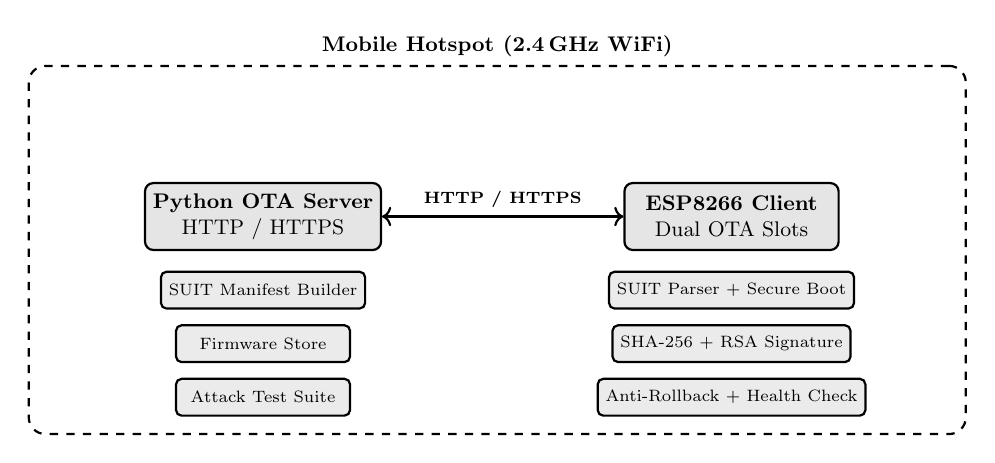
\begin{tikzpicture}[
  box/.style={draw, thick, rounded corners=3pt, minimum height=1cm,
              minimum width=3.2cm, align=center, font=\small},
  comp/.style={draw, thick, rounded corners=2pt, minimum height=0.55cm,
               minimum width=2.6cm, align=center, font=\scriptsize,
               fill=black!8},
  arr/.style={-{Stealth[length=3mm]}, thick},
  scale=0.85, transform shape
]

% Hotspot
\node[draw, dashed, thick, rounded corners=6pt,
      minimum width=14cm, minimum height=5.5cm,
      label={[font=\small\bfseries]above:Mobile Hotspot (2.4\,GHz WiFi)}] (hotspot) {};

% Server
\node[box, fill=black!10] (server) at (-3.5, 0.5) {\textbf{Python OTA Server}\\HTTP / HTTPS};
\node[comp] (manifest) at (-3.5, -0.6) {SUIT Manifest Builder};
\node[comp] (fwstore) at (-3.5, -1.4) {Firmware Store};
\node[comp] (edgetest) at (-3.5, -2.2) {Attack Test Suite};

% Device
\node[box, fill=black!10] (device) at (3.5, 0.5) {\textbf{ESP8266 Client}\\Dual OTA Slots};
\node[comp] (parser) at (3.5, -0.6) {SUIT Parser + Secure Boot};
\node[comp] (sha) at (3.5, -1.4) {SHA-256 + RSA Signature};
\node[comp] (rollback) at (3.5, -2.2) {Anti-Rollback + Health Check};

% Arrows
\draw[arr, <->] (server.east) -- node[above, font=\scriptsize\bfseries] {HTTP / HTTPS} (device.west);

\end{tikzpicture}

\vspace{4pt}
{\small\textbf{Three-Tier:} Mobile Hotspot $\rightarrow$ Python OTA Server (Laptop) $\rightarrow$ ESP8266 Client}

\end{frame}

% ══════════════════════════════════════════════════════════════════
%  SLIDE 6 — Secure Update Pipeline
% ══════════════════════════════════════════════════════════════════
\begin{frame}{Secure Update Pipeline}

\centering
\begin{tikzpicture}[
  step/.style={draw, thick, rounded corners=2pt, minimum height=0.6cm,
               minimum width=5cm, align=center, font=\scriptsize,
               fill=black!6},
  arr/.style={-{Stealth[length=2mm]}, thick},
  scale=0.78, transform shape
]

\node[step] (s1) at (0,0) {1. WiFi Connection (WPA2-PSK)};
\node[step] (s2) at (0,-0.9) {2. Fetch SUIT Manifest (HTTP/HTTPS)};
\node[step] (s3) at (0,-1.8) {3. Validate Manifest (Magic Bytes)};
\node[step] (s4) at (0,-2.7) {4. Anti-Rollback Check};
\node[step] (s5) at (0,-3.6) {5. Signature / Secure Boot Verify};

\node[step] (s6) at (8,-0) {6. Download Firmware (HTTP/HTTPS)};
\node[step] (s7) at (8,-0.9) {7. SHA-256 Integrity Check};
\node[step] (s8) at (8,-1.8) {8. Flash to Inactive OTA Slot};
\node[step] (s9) at (8,-2.7) {9. Health Check + Reboot};

\foreach \i/\j in {s1/s2, s2/s3, s3/s4, s4/s5, s6/s7, s7/s8, s8/s9} {
  \draw[arr] (\i) -- (\j);
}
\draw[arr] (s5.east) -- ++(1.2,0) |- (s6.west);

\end{tikzpicture}

\vspace{6pt}
{\small Any step failure $\Rightarrow$ \textbf{firmware rejected}, device remains on current version.}

\end{frame}

% ══════════════════════════════════════════════════════════════════
%  SLIDE 7 — Secure Boot + Hardware Root of Trust
% ══════════════════════════════════════════════════════════════════
\begin{frame}{Secure Boot + Hardware Root of Trust}

\begin{columns}[T]
\column{0.48\textwidth}
\begin{block}{Boot Chain}
\centering
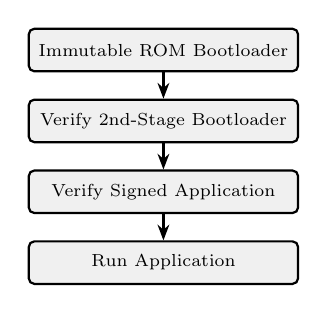
\begin{tikzpicture}[
  box/.style={draw, thick, rounded corners=2pt, minimum height=0.6cm,
              minimum width=3.8cm, align=center, font=\scriptsize, fill=black!6},
  arr/.style={-{Stealth[length=2mm]}, thick},
  scale=0.9, transform shape
]
\node[box] (rom) at (0,0) {Immutable ROM Bootloader};
\node[box] (bl2) at (0,-1) {Verify 2nd-Stage Bootloader};
\node[box] (app) at (0,-2) {Verify Signed Application};
\node[box] (run) at (0,-3) {Run Application};
\draw[arr] (rom) -- (bl2);
\draw[arr] (bl2) -- (app);
\draw[arr] (app) -- (run);
\end{tikzpicture}
\end{block}

\column{0.48\textwidth}
\begin{block}{Technologies}
\begin{itemize}\small
  \item ESP32 Secure Boot v2
  \item ROM bootloader as trust anchor
  \item RSA-PSS digital signatures
  \item eFuse-based key storage
\end{itemize}
\end{block}

\vspace{4pt}
\begin{block}{Protection}
\begin{itemize}\small
  \item Modified firmware cannot execute
  \item Trust anchored below application layer
  \item Stronger than software-only checks
\end{itemize}
\end{block}
\end{columns}

\end{frame}

% ══════════════════════════════════════════════════════════════════
%  SLIDE 8 — Flash Encryption + Secure Transport
% ══════════════════════════════════════════════════════════════════
\begin{frame}{Flash Encryption + Secure Transport}

\begin{columns}[T]
\column{0.48\textwidth}
\begin{block}{Flash Encryption}
\begin{itemize}\small
  \item Protects firmware stored in off-chip flash
  \item Hardware-supported encryption (AES)
  \item Prevents physical flash reading attacks
  \item Used together with Secure Boot
\end{itemize}
\end{block}

\vspace{4pt}
\begin{block}{HTTPS / TLS}
\begin{itemize}\small
  \item OTA downloads via \texttt{esp\_https\_ota}
  \item TLS protects firmware in transit
  \item Not a replacement for signing
\end{itemize}
\end{block}

\column{0.48\textwidth}
\begin{block}{Three Security Layers}
\centering
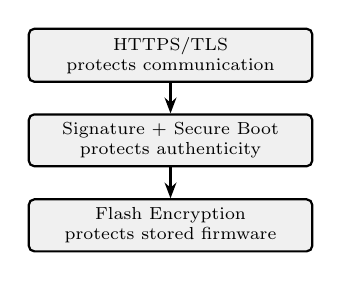
\begin{tikzpicture}[
  box/.style={draw, thick, rounded corners=2pt, minimum height=0.7cm,
              minimum width=4cm, align=center, font=\scriptsize, fill=black!6},
  arr/.style={-{Stealth[length=2mm]}, thick},
  scale=0.9, transform shape
]
\node[box] (tls) at (0,0) {HTTPS/TLS\\protects communication};
\node[box] (sig) at (0,-1.2) {Signature + Secure Boot\\protects authenticity};
\node[box] (enc) at (0,-2.4) {Flash Encryption\\protects stored firmware};
\draw[arr] (tls) -- (sig);
\draw[arr] (sig) -- (enc);
\end{tikzpicture}
\end{block}
\end{columns}

\end{frame}

% ══════════════════════════════════════════════════════════════════
%  SLIDE 9 — OTA + Health Check + Rollback
% ══════════════════════════════════════════════════════════════════
\begin{frame}{A/B OTA + Health Check + Rollback}

\begin{columns}[T]
\column{0.48\textwidth}
\begin{block}{OTA Architecture}
\begin{itemize}\small
  \item \texttt{OTA\_0} = V1 known-good firmware
  \item \texttt{OTA\_1} = V2 candidate firmware
  \item OTA data partition tracks boot state
  \item Download via \texttt{esp\_https\_ota} over TLS
  \item V2 stored in inactive slot (V1 preserved)
\end{itemize}
\end{block}

\column{0.48\textwidth}
\begin{block}{Health Check}
\begin{itemize}\small
  \item Signed firmware can still have bugs
  \item Secure Boot $\neq$ ``firmware works''
  \item Self-tests after first V2 boot:
    \begin{itemize}\scriptsize
      \item Peripherals initialize
      \item WiFi/network connects
      \item Critical services start
    \end{itemize}
  \item \textbf{Pass} $\rightarrow$ mark V2 valid
  \item \textbf{Fail} $\rightarrow$ rollback to V1
\end{itemize}
\end{block}
\end{columns}

\vspace{6pt}
\centering
{\small\textbf{Secure Boot} = ``Is this authorized?'' \quad\textbf{Health Check} = ``Does it work?'' \quad\textbf{Rollback} = ``How do we recover?''}

\end{frame}

% ══════════════════════════════════════════════════════════════════
%  SLIDE 10 — Security Mechanisms Summary
% ══════════════════════════════════════════════════════════════════
\begin{frame}{Security Mechanisms}

\renewcommand{\arraystretch}{1.25}
\begin{table}
\centering
\small
\begin{tabular}{l l l}
\toprule
\textbf{Feature} & \textbf{Implementation} & \textbf{Standard} \\
\midrule
Integrity & SHA-256 & NIST FIPS 180-4 \\
Authentication & RSA digital signatures & PKCS\#1 / RFC 8017 \\
Secure Boot & Hardware root of trust (eFuse) & ESP32 Secure Boot v2 \\
Flash Encryption & AES hardware encryption & ESP32 Flash Encrypt \\
Manifest Validation & Magic bytes + field bounds & SUIT (simplified) \\
Device Authorization & X-Device-ID HTTP header & Custom (server-side) \\
Secure Transport & HTTPS / TLS & TLS 1.2+ \\
\bottomrule
\end{tabular}
\end{table}

\end{frame}

% ══════════════════════════════════════════════════════════════════
%  SLIDE 11 — Demo Tests / Attack Matrix
% ══════════════════════════════════════════════════════════════════
\begin{frame}{Demo Tests \& Attack Matrix}

\renewcommand{\arraystretch}{1.15}
\begin{table}
\centering
\small
\begin{tabular}{c l l}
\toprule
\textbf{\#} & \textbf{Attack / Test Scenario} & \textbf{Expected Result} \\
\midrule
1 & Valid signed V2 firmware & V2 boots, passes health check \\
2 & Modified V2 (tampered binary) & Secure Boot rejects, V1 remains \\
3 & Unsigned V2 firmware & Rejected at signature check \\
4 & Older firmware (rollback attempt) & Anti-rollback rejects it \\
5 & Signed but buggy V2 & Health check fails, rollback to V1 \\
6 & Flash read attempt & Flash Encryption protects contents \\
\midrule
7 & Corrupt hash in manifest & SHA-256 mismatch, rejected \\
8 & Bad magic bytes (\texttt{0xDEADBEEF}) & Manifest validation fails \\
9 & Unauthorized device ID & Server denies firmware \\
\bottomrule
\end{tabular}
\end{table}

\vspace{4pt}
\centering
All tests must result in \textbf{CORRECTLY REJECTED} (except test 1) for a passing score.

\end{frame}

% ══════════════════════════════════════════════════════════════════
%  SLIDE 12 — Hardware \& Software Setup
% ══════════════════════════════════════════════════════════════════
\begin{frame}{Hardware \& Software Setup}

\begin{columns}[T]
\column{0.48\textwidth}
\begin{block}{Hardware}
\small
\begin{tabular}{l l}
\toprule
\textbf{Spec} & \textbf{Detail} \\
\midrule
MCU & NodeMCU ESP8266 (Only MCU used) \\
CPU & Tensilica L106 32-bit (80\,MHz) \\
Flash & 4\,MB SPI Flash \\
WiFi & 802.11 b/g/n (2.4\,GHz) \\
\bottomrule
\end{tabular}
\end{block}

\column{0.48\textwidth}
\begin{block}{Software Stack}
\small
\begin{tabular}{l l}
\toprule
\textbf{Layer} & \textbf{Technology} \\
\midrule
Server & Python HTTP Server \\
Protocol & HTTP / HTTPS \\
Signatures & RSA \\
Integrity & SHA-256 \\
\bottomrule
\end{tabular}
\end{block}
\end{columns}

\end{frame}

% ══════════════════════════════════════════════════════════════════
%  SLIDE 13 — Summary \& Contribution
% ══════════════════════════════════════════════════════════════════
\begin{frame}{Summary \& Contribution}

\begin{block}{What We Built}
A complete, secure OTA firmware update system that evolved from a software-only ESP8266 prototype to a hardware-backed ESP32 solution.
\end{block}

\vspace{6pt}
\begin{columns}[T]
\column{0.48\textwidth}
\begin{block}{Completed Work (ESP8266 Baseline)}
\begin{itemize}\small
  \item SUIT manifest, SHA-256, RSA
  \item V1/V2 rollback, device authorization
\end{itemize}
\end{block}

\column{0.48\textwidth}
\begin{block}{Proposed Work (ESP32 Extension)}
\begin{itemize}\small
  \item Secure Boot v2 (hardware trust)
  \item Flash Encryption (AES)
  \item HTTPS/TLS transport
  \item A/B OTA + health check recovery
\end{itemize}
\end{block}
\end{columns}

\vspace{8pt}
\centering
\textit{``We retained the old rollback system and added hardware-enforced boot trust, encrypted storage, and secure transport --- making the complete firmware-update system more secure and resilient.''}

\end{frame}

\end{document}
